\chapter{Generators in Peachpie}

The goal of this thesis is to enable Peachpie compiler to handle PHP generator methods while keeping as much of their original semantics as possible. That means we do not want to change their behavior and want to enable all the features they offer in PHP, only now compiled to CIL and executed either by the CLR or another CLI environment.
 
As noted in previous chapters\footnote{Chapter \ref{sec:3:1}}, this in itself is complicated, because unlike the PHP runtime Zend Engine, the CIL and CLR do not have a native support for generators or generally pausing the execution of a method at arbitrary points. Also, almost all other CIL based languages with generators, such as C\# or F\#, that implement them by compiler transformations have them in a substantially more limited form than PHP.

Other than that, we also want to reuse existing Peachpie infrastructure and only implement generator specific bits when necessary. While this goal is not as important for our immediate work, it is necessary for the project as a whole. Cluttering the compiler with logic for a feature that is not actually used as often would simply be inexcusable.

\section{Basic generators implementation}

Before dealing with all the complexities of PHP’s generators, let us first explore how an implementation of their limited subset would work within Peachpie. Specifically, we will ignore \emph{yield} in exception handling blocks and expect it to be only in places where it could happen as a statement, i.e. no \emph{yield} inside an expression tree, for this chapter. 

Much like Roslyn’s approach, our implementation of generators within Peachpie will also be based on transforming the original generator method into an iterator's \emph{next} method. So as not to repeat ourselves, we will only point out the differences in the next section.

\subsection{Iterator object}

Unlike in C\#, where generator methods are free to return any object implementing an \emph{IEnumerator} interface, the PHP specification dictates that the returned object must be an instance of a \emph{Generator} type \citep{GenPHP, GenPHPRFC}. This means that in Peachpie we cannot just synthesize a new type for each generator method as Roslyn does.

If we were to do that, all reflection methods and type checks would report the actual synthesized type on the returned iterator instance instead of the \emph{Generator} type, as required by PHP’s specification . We could theoretically hard code exceptions for these synthesized types into all methods that query an instance’s type, but that would go against our goal to implement as little feature specific code as possible.

Instead, we must create one generator type in Peachpie’s runtime library and use it as a basis for all generator methods to return. That approach, however, carries some limitations with it. The generator type can now include only shared code and fields. That means neither a specific \emph{next} method’s implementation nor fields for lifted local variables from said method.

Other than that, the \emph{Generator} type can be practically the same as the ones synthesized by Roslyn as it is a simple implementation of PHP's \emph{Iterator} interface (\autoref{list5.1:GeneratorType}). It can hold a captured reference to the \emph{this} instance of the original generator method, a state field to know what point the \emph{next} method should continue from,  fields for the \emph{current} element and, since we are in PHP now, its \emph{key}.

\begin{listing}[H]
\caption{Simplified version of the Generator type.}
\label{list5.1:GeneratorType}
\begin{minted}{csharp}
public delegate void GeneratorStateMachineDelegate(
  Context ctx, object @this, PhpArray locals, 
  Generator gen);
public class Generator : Iterator
{
  readonly Context _ctx;
  readonly GeneratorStateMachineDelegate _stateMachineMethod;
  readonly object _this;
  readonly PhpArray _locals;
  internal int _state = 0;
  internal PhpValue _currValue, _currKey;
  public void next() =>
  _stateMachineMethod.Invoke(_ctx, _this, _locals, gen: this);
}
\end{minted}
\end{listing}

\subsection{Next method implementation and local variables}

The \emph{next} method's implementation problem is easily solvable. The shared generator type can hold a delegate to an implementation of the \emph{next} method instead of the method itself. This enables Peachpie compiler to synthesize the \emph{next} method anywhere and then to assign its delegate to the generator. The generator must still implement some \emph{next} method to comply with the Iterator interface but it can be a shim that only calls the saved delegate.

There is only one restriction with regards to the actual \emph{next} method’s placement. The transformed method must be accessible from within the original generator method. The reason is that the original method is where the instantiation and initialization of the generator, thus also the creation and assigning of the delegate, happens. 

One such suitable place is the enclosing type of the original method, where it can always be synthesized as a static method. It being a static method is not a problem because, as mentioned in the chapter about Roslyn’s implementation, a reference to the enclosing type’s instance is passed as a \emph{this} parameter. And since the enclosing type could be a static class, it cannot be a normal instance method anyway.

The inability to add fields to the generator type can also be overcome. As described in the CIL emit phase chapter\footnote{Chapter \ref{CodeGen}}, Peachie's \emph{CodeGenerator} supports specifying where local variables should live within a method with the option to, for example, move them to a \emph{PhpArray}.

With that, a \emph{PhpArray} field can be added to the generator type and we can specify that all of the \emph{next} method's local variables should live on it. Because parameters are considered local variables in Peachpie, this approach handles them as well. They only need to be initialized with their values in the original generator method. That way, the \emph{next} method’s local variables and parameters get lifted to the generator type the same way as in Roslyn, with the only difference being that they do not get lifted to individual fields but to a single \emph{PhpArray} (\autoref{fig5.1:Generator}).

\subsection{Accessibility of fields on the Generator type}

Moving the \emph{next} method outside of the generator type means that the method cannot access its fields such as \emph{current} or state directly through a \emph{this} reference. That is a problem, because the method needs to both read and write these fields to progress the generator. An effective solution is to pass the generator instance as a parameter through the \emph{next} method delegate - in essence to not only call the delegate from within the generator’s own \emph{next} method, but to call it with a \emph{this} reference as a parameter.

That on its own would be enough if all the fields on the generator type were public. That is, however, not our objective. We want the generator type to have the same public API as it does in PHP and there are no such public fields in PHP’s \emph{Generator}. Therefore, we need to find a way to access the fields from a method within the user’s assembly, the transformed \emph{next} method the generator has a delegate to, without having to make the fields accessible to other user code.

One way to do this is to make the generator fields internal and create public getter and setter methods for these fields in the Runtime library. Since the generator type also lives there, the methods can access its fields and, because they are public, they can be used from within the synthesized \emph{next} method (\autoref{fig5.1:Generator}). The methods can be simple static getters and setters, always taking a generator instance as a first parameter and either returning an appropriate field’s value or taking its value as a second parameter and then setting it on the instance.

\begin{figure}[h]
	\centering	
	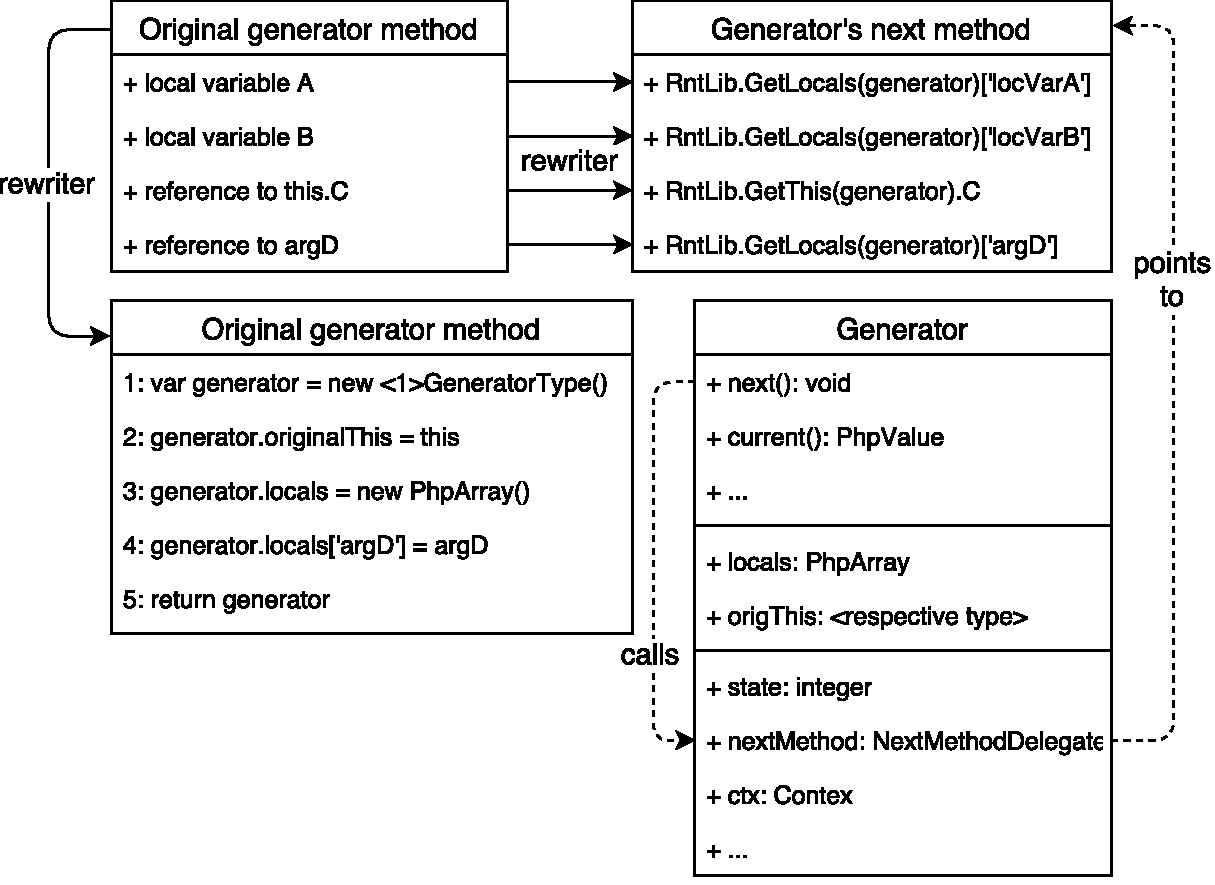
\includegraphics[scale=0.70]{../img/5_1_Generator}	
	\caption{Transformation of the generator method.}
	\label{fig5.1:Generator}
\end{figure}

While it is true that this approach still opens a way for the user to modify the generator’s internal state, it has to be done through special methods from Peachpie runtime library and as such, it can hardly be done by accident. It also ensures a compliant public API of the \emph{Generator} type.

\subsection{Context handling}

Being in PHP, we need to ensure that the correct PHP \emph{Context} gets passed to our moved \emph{next} method. There are two ways to do it. Current \emph{context} can either be passed as part of each call to the generator methods, and subsequently via a delegate to the \emph{next} method, or it can be captured once during the generator’s initialization and then reused the same way as is the \emph{this} instance.

Neither approach is inherently wrong. Passing the \emph{context} with each call ensures the current one is used even in situations where one generator instance is used with multiple PHP \emph{context}s. That can happen, for example, when PHP code is called from some other .NET language and multiple \emph{context}s are created manually. This approach is also more in line with how \emph{context} on normal instances is handled. It is not captured in the constructor and then used by all the instance methods, but always passed as a parameter.

On the other hand, capturing the \emph{context} on the generator’s creation better represents the idea that the generator is a fully self-contained object. It is also marginally easier to implement and provides better opportunities for interop between PHP generators and other .NET languages. This way, a generator can be created in PHP and then used elsewhere as a normal iterator, without having to explicitly keep and supply its \emph{context}. Thus, the capture once in the original generator method approach was chosen.

\subsection{Rewriter}

Due to architectural differences, we will not have a standalone rewriter component in Peachpie. While it would be possible, there are, as of writing this thesis, no other candidates that could make use of them within the compiler. And adding a generic support just to have one rewriter for generators goes against our goal to keep the implementation as simple as possible. Instead, our implementation will rely on support by the \emph{SemanticBinder}, slightly changed emit of a \emph{MethodSymbol} and \emph{StartBlock}\footnote{Chapter \ref{StartBlock}}, and a new semantic node. 

As long as we limit ourselves to \emph{yield} only at places where it could be as a statement, which is the temporal restriction we have set for this chapter, the support provided by the \emph{SemanticBinder} can be minimal. It needs to do two things: bind the new semantic object - \emph{BoundYieldExpression} - when it encounters the AST’s \emph{YieldExpression} and mark the method’s symbol as a generator. 

\subsection{Bound yield expression}

The \emph{BoundYieldExpression} can be a rather simple semantic node with two children: the yielded key and yielded value expressions. It should generate CIL to set the yielded key and value fields on the generator instance, update its state, \emph{return}, and mark a label for the subsequent continuation (\autoref{fig5.1:Rewriter}). 

Due to being an expression, albeit for this chapter limited to places where it could also be a statement, it needs to push and leave its value on the evaluation stack. However, since its value will not be needed due to our restriction, it can just as well be an empty \emph{PhpValue}. The value will always get discarded, anyway. The restriction also handles the problem that we are emitting a \emph{return} from within an expression, i.e. in a situation in which the evaluation stack might not be empty.

It is true that all of the \emph{BoundYieldExpression} could be replaced with a number of normal PHP statements by lowering. That would, however, require the \emph{SemanticBinder} to be able to produce multiple semantic statements for only one AST node, and for the \emph{BuilderVisitor} to accept them. And while such support could be added, it was decided that it would be too complex.

\begin{figure}[h]
	\centering	
	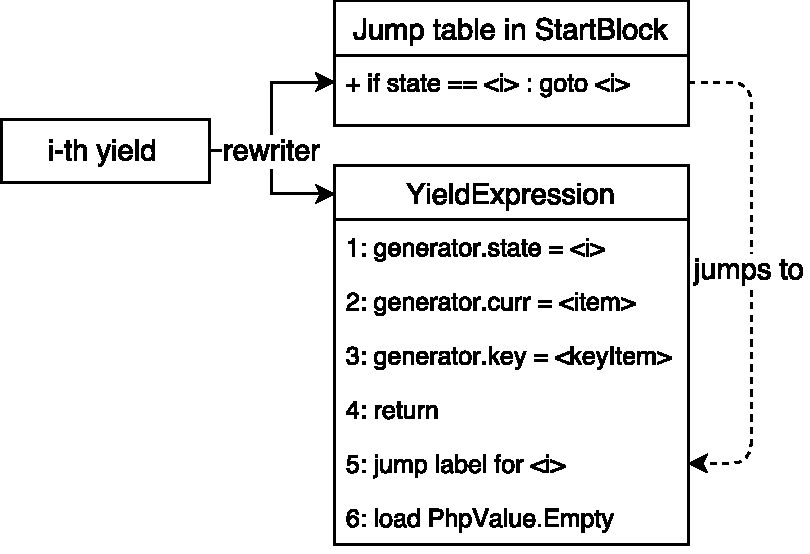
\includegraphics[scale=0.75]{../img/5_1_rewriter}	
	\caption{Rewrite of a yield expression.}
	\label{fig5.1:Rewriter}
\end{figure}


\subsection{Start block}\label{StartBlock}

The \emph{StartBlock} is a special instance of a \emph{BoundBlock} that is present in the beginning of each method’s control flow graph (\autoref{fig3.4:EmitOrder}). As such, its emit routine is the perfect place to generate a jump table for generator methods. It can, when its enclosing method symbol is a generator, query all present \emph{yield} statements that were previously set by, for example, the semantic binder and generate the whole jump table.

\subsection{Method symbol}\label{MethdSymbol}

The method symbol’s emit must be changed as well. When it represents a generator, it cannot simply generate the CIL representation of its body. If it did that, it would not produce a method that returns an iterator as it should, but a method that implements the iterator’s \emph{next} method.

Instead, three things need to happen. First, a new static method representing the generator’s \emph{next} method must be synthesized in the enclosing type. Second, the original body needs to be emitted inside the synthesized method with its \emph{CodeGenerator} set to offload local variables into a generator’s locals field. As explained earlier, the synthesized \emph{next} method accepts a \emph{Generator} as a parameter.

Third, a sequence of statements that create, initiate, and \emph{return} a \emph{Generator} instance must be emitted as the actual current method symbol’s body, producing a method that returns an iterator. As part of the initiation phase a delegate to the synthesized \emph{next} method must get created and assigned to the newly constructed generator instance. Also, values of all parameters need to get copied to the generator’s locals array, as previously discussed.

\section{Yield as an expression - theory}\label{AlghTheory}

With that, we have described a design of a generator’s compilation within the Peachpie platform with a featureset limited to more or less C\# generators. Now, let us broaden it with the support for \emph{yield} as an expression. Before going into details on the specific implementation, let us first take a look at the general idea behind our approach. 

As said before, a \emph{yield} being an expression is a problem, because an expression can happen in a situation where the CIL evaluation stack might not be empty. Since \emph{yield}s include a \emph{return} and returning with a non-empty evaluation stack is forbidden, it does not go well together. Even if it were allowed, there would still be the problem that the non-empty evaluation stack would represent some sort of state - one that would need to get saved and then retrieved upon the continuation.

\subsection{Possible approaches}

Fundamentally, there are two possible ways to approach this problem. One can either come up with a mechanism to save and then retrieve the evaluation stack or rearrange the semantic graph so that \emph{yield}s are only in places where they could happen as statements.

While the first approach might be appealing, after all it more closely mimics the Zend Engine’s way of handling yields\footnote{Chapter \ref{ZendGen}}, it is almost impossible to implement. Because the CIL does not have any instructions to query the contents or to completely save/load the evaluation stack, the compiler would have to do it manually. That means it would have to track the stack’s content throughout the compilation and then emit individual instructions to save/load its content, one element at a time.

That would mean two things. First, we would either have to create our own version of the \emph{CodeGenerator} that would be able to keep track of what the evaluation stack contains at any moment or we would have to change the emit of each semantic node to save the information about what it puts on the stack explicitly. Both of these would be relatively complex to do and, in case of the second approach, even to maintain due to possible new semantic nodes. Second, either of them would mean an increase in memory usage because we would need to remember information previously not required, all of which just to support only a \emph{yield} as an expression. 

On the other hand, the second approach, to rearrange the semantic tree, requires only a few local implementation changes and does not cause a substantial memory consumption increase. Essentially, it is based on the idea that we can break an expression tree into a series of statements while keeping the meaning and order of execution the same.

\subsection{Branch capture \& yield splitting}

There are two important observations required for this method. First, a \emph{yield} can be broken into two semantic nodes. A statement that does the value and key setting, state saving, \emph{return}, and marking the continuation label, acting as the equivalent of a C\# \emph{yield} statement. The other node is an expression that represents the sent value. If the expression directly follows the statement, the result is, in terms of emitted CIL, the same as with one combined \emph{yield expression} (\autoref{fig5.2:Splitting}). 


\begin{figure}[h]
	\centering	
	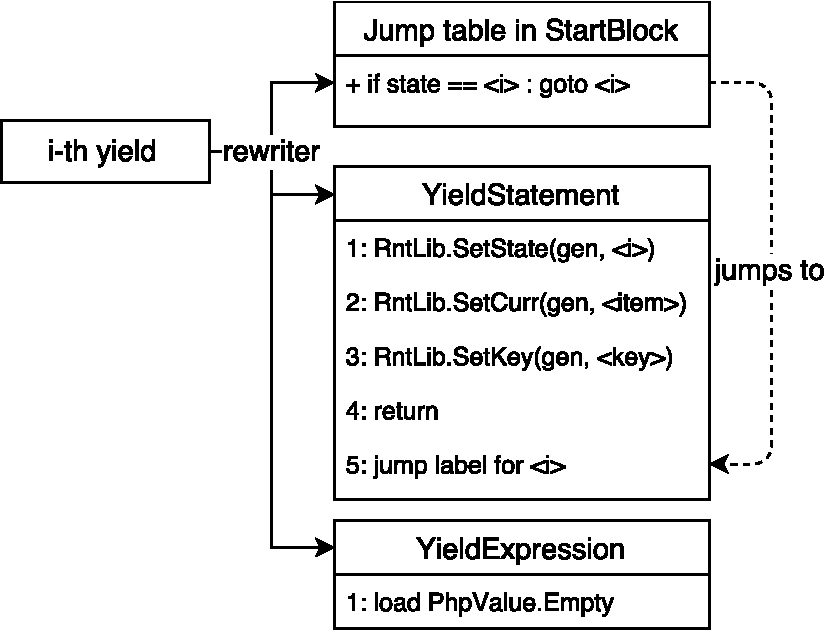
\includegraphics[scale=0.75]{../img/5_2_yieldSplitting}	
	\caption{Splitting of a yield into an expression and a statement.}
	\label{fig5.2:Splitting}
\end{figure}

Second, we can cut any branch in an expression tree and prepend it before the tree while keeping the meaning of the program the same except for the order of execution. To do it, we need to create a temporal variable, replace the branch in the tree with a read from said variable, and prepend the tree with a statement that assigns the branch that was replaced to the variable it was replaced with (\autoref{fig5.2:CaptureBranch}). Let us call this process capturing a branch.

The problem with the order of execution is that the captured branch, being lifted to the prepended statement, will get executed before any other expression from the tree. Even before all the expressions in branches that might be to the left of the captured branch and that were therefore supposed to be executed first. In the figure below, the expressions $5$ and $6$ respectively will get executed first, even though they should come after expressions $1$, $2$, $3$, and $4$.


\begin{figure}[h]
	\centering	
	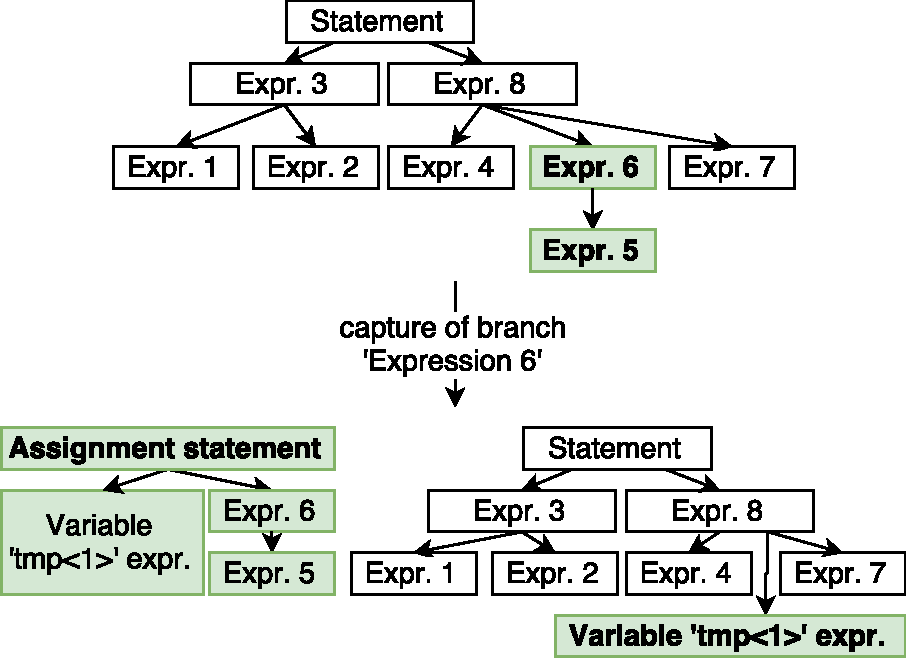
\includegraphics[scale=0.75]{../img/5_2_capturing}	
	\caption{Capturing a sole branch.}
	\label{fig5.2:CaptureBranch}
\end{figure}

An obvious solution to this problem is to cut and prepend not only the one branch we want to capture, but also, in their respective order from left to right, all other branches that are supposed to get executed before it (\autoref{fig5.2:CaptureAllBranch}). Since the semantic graph emit, and thus also the execution, follows a post-order traversal, we must cut and prepend all branches that are higher and to the left of the branch we want to capture. 

To be specific, that includes all branches that start to the left of the path between the root of our captured branch and the root of the whole semantic graph. The reason lies in a post-order traversal of the semantic graph. 

It starts with the graph’s root. Then it goes through the root’s leftmost child, followed by its next child, and so on. Let us say, for example, that the second element of our aforementioned path is the root’s third child. When the traversal enters it after going through the branches started by the root’s first two children, it goes into its leftmost child first, again. It then continues the same way until it encounters the root of our branch. When that happens, it keeps following the same logic, traversing the whole branch before closing its root and starting to visit any other nodes. After the traversal is finished with the branch, it closes its root and goes one level up, starting to traverse the branch’s root’s first sibling to the right.   

All other expressions, be it those directly on the path or on branches to the right, are supposed to be evaluated after our branch and, as such, do not have to be cut and prepended. The ones on the path have our branch among their children and thus need its result - our branch - to be evaluated first. And the ones on the right need to be evaluated later, simply because of post-order traversal rules. 

\begin{figure}[h]
	\centering	
	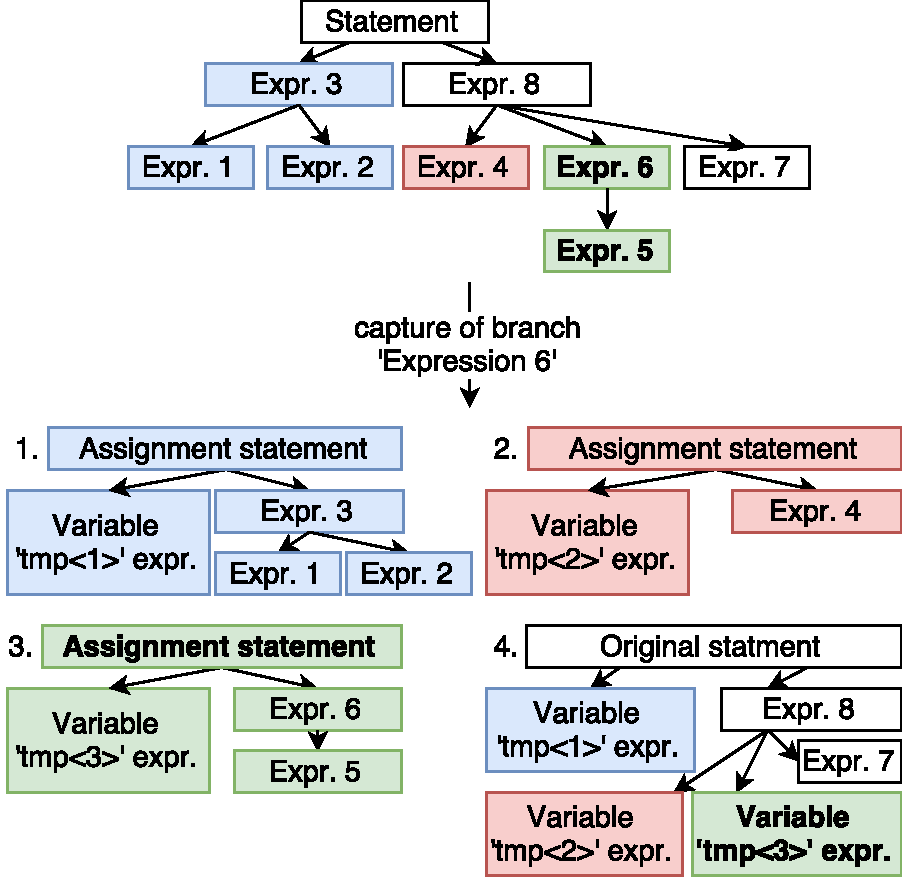
\includegraphics[scale=0.75]{../img/5_2_captureAllOnPath}	
	\caption{Capturing a whole branch while maintaining execution order.}
	\label{fig5.2:CaptureAllBranch}
\end{figure}

\subsection{Semantic tree transformation}

Now we can combine the two observations from the beginning of the previous section and come up with a solution to our \emph{yield} as an expression problem. Our goal is to split each \emph{yield} and then separate its statement part while maintaining the original order of execution.

To be able to do it, the \emph{yield} has to be on top of an expression tree first. It must be, in terms of execution order, its first user code representing node. When that is true, we can split the \emph{yield} into a \emph{yield expression} and a \emph{yield statement}, and then put the statement part before the tree. 

This does not change the program’s meaning or order of execution, because the \emph{yield statement} is directly followed by the tree and the tree’s first user code node is the \emph{yield} expression. And since the part of the \emph{yield} containing a \emph{return} is a proper statement before - not inside - a tree, the semantic graph is actually emitable.

With that, our problem has shifted to transforming expression trees containing \emph{yield}s at arbitrary places into multiple expression trees that have them only as their first user code representing nodes. If we were able to do that, we could split each of the \emph{yield}s and separate their \emph{return} containing parts as standalone statements.

The transformation can be done through our branch capturing mechanism. We can take each branch that starts with a \emph{yield} and capture it (\autoref{fig5.2:CaptureYield}). That prepends its tree with an assignment of the captured branch and all other branches that are, within the tree, supposed to get executed before it. None of the other branches are of significance for us, so let us ignore them and focus only on the captured one. 

The tree representing a prepended assignment of the capture branch contains a \emph{yield} as its first expression that is not the synthesized \emph{assignment statement} itself. This holds true, because we specifically captured a branch that starts with a \emph{yield}. As such, the tree representing the prepended branch fully adheres to our requirements for splitting the \emph{yield} into a statement and an expression.

\begin{figure}[h]
	\centering	
	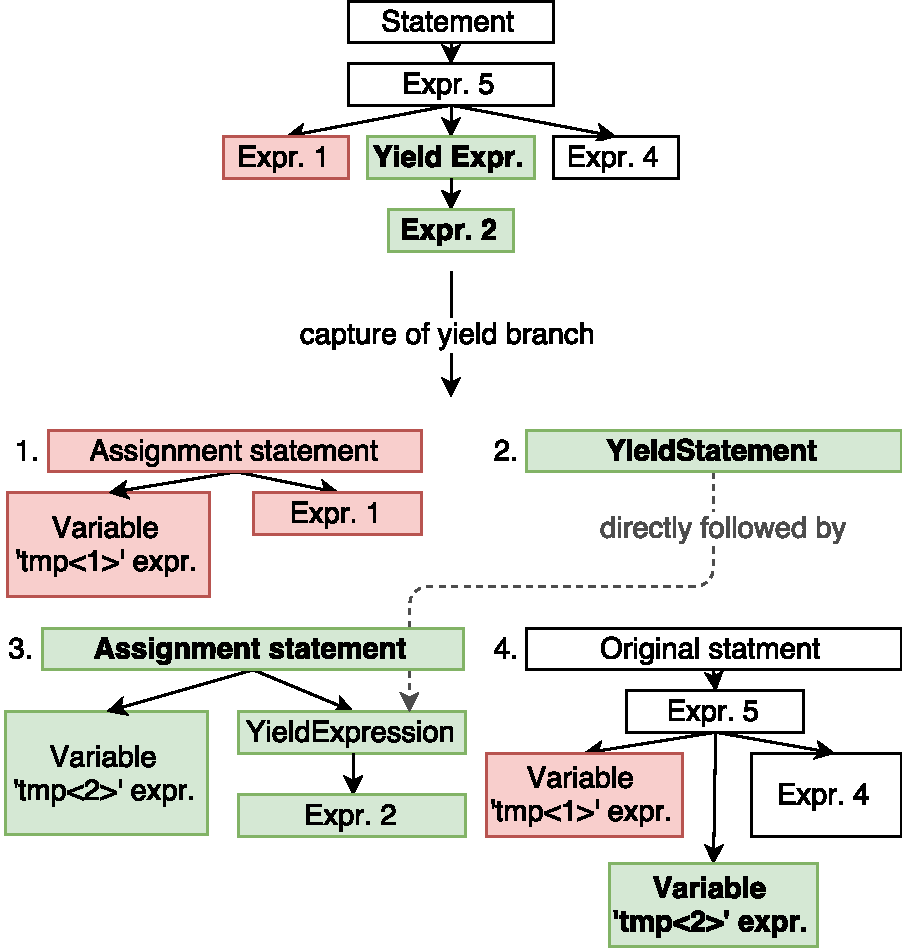
\includegraphics[scale=0.75]{../img/5_2_yieldCapturing}	
	\caption{Capturing a whole branch starting with a yield.}
	\label{fig5.2:CaptureYield}
\end{figure}

Now we have to repeat the aforementioned process for each expression tree containing \emph{yield}s and for each of their branches that starts with them. Every run of our algorithm fixes one \emph{yield} and results in a correct semantic graph that can serve as a starting point for another run. This means that after a finite number of repetitions, all \emph{yield}s will have been split while keeping the original program’s meaning and execution order intact.

\subsection{Short circuit evaluation}

The solution from the previous section would work perfectly, if it were certain that all branches of an expression tree will always get evaluated. The problem is, that they do not. For example, a conditional operator \emph{? :} is represented by an expression that has three children, only two of which get evaluated in any given situation. Its children are a \emph{condition expression} that gets evaluated first and every time, and two \emph{conditioned expression}s representing its return value. One, that gets evaluated and returned when the condition turns out to be true, and one, for when it is false. A similar situation transpires with short-circuit evaluated binary expressions such as coalesce, and, and or operators.

The problem is, that a \emph{yield} can be inside one of these \emph{conditioned branches} and when its gets captured and prepended before the tree, it will always get executed regardless of the \emph{condition}. For example, even if the \emph{condition} were false, an expression tree for its true branch, being prepended before the tree because it includes a \emph{yield}, would still get executed and had its result saved into a temporal variable. The variable would simply not get used as a result of the \emph{condition expression} (\autoref{list5.3:CondNotGuarded}).

\begin{listing}[H]
\caption{Conditional expression whose captured branch is not conditioned.}
\label{list5.3:CondNotGuarded}
\begin{minted}{php}
<?php
// Original expression before capturing the yield branch.
$result = isTrue() ? yield 0 : "falseBr";

// Expression with a captured yield branch.
$tmpBranch = yield 0; // The yield is evaluated everytime.
$result = isTrue() ? $tmpBranch : "falseBr";
\end{minted}
\end{listing}

This, of course, represents a problem. While the result of each expression would remain correct, a whole expression branch would now get executed every time instead of only when a certain condition was satisfied. And even if the branch itself did not have any side effects, it starts with a \emph{yield} which includes a \emph{return}. A \emph{return} that was previously conditioned but is now executed every time.

Fortunately, the solution is relatively simple. When going through the semantic graph to capture branches starting with a \emph{yield}, the mechanism can remember when it enters and leaves a \emph{conditioned branch}. And when it is about to capture a sub-branch while being in a \emph{conditioned branch}, it can simply not prepend its assignment as described previously. Instead, it can prepend a \emph{condition edge} that has the \emph{assignment statement} in its true block and a logical conjunction of all conditions guarding the current branch as its \emph{condition expression} (\autoref{list5.3:CondTwice}). That way, the prepended assignment with the captured branch will get executed only when the condition is true, in essence in the same situations in which it, at its original position, in the tree would.

\begin{listing}[H]
\caption{Conditional expression whose condition is evaluated twice.}
\label{list5.3:CondTwice}
\begin{minted}{php}
<?php
// The condition `isTrue()` is evaluated twice.
if isTrue() { $tmpBranch = yield 0; }
$result = isTrue() ? $tmpBranch : "falseBr";
\end{minted}
\end{listing}

Unfortunately, that in itself is still not enough. With that reuse, each \emph{condition expression} is possibly evaluated multiple times. Once as the original expression in the tree and once for each \emph{condition edge} created by capturing a sub-branch from the \emph{conditioned branch}. Even this problem has a straightforward solution.

One can capture each branch representing a \emph{condition expression} whose respective \emph{conditioned branches} are to be captured in the future, i.e. that include a \emph{yield}. Subsequently, one can use the temporal variable created by the capture instead of the expression itself in both the \emph{condition edge}s and its original location in the tree (\autoref{list5.3:CondCorrect}). That way, the \emph{condition expression} gets evaluated only once as part of a prepended assignment and its result is reused. And because the capturing also prepends all branches that are before the \emph{condition expression} in the tree, the order of execution stays the same. 

\begin{listing}[H]
\caption{Conditional expression captured correctly.}
\label{list5.3:CondCorrect}
\begin{minted}{php}
<?php
$tmpCond = isTrue(); // Condition expression is evaluated once.
if ($tmpCond) { $tmpBranch = yield 0; }     //`tmpCond` is reused.
$result = $tmpCond ? $tmpBranch : "falseBr";//`tmpCond` is reused.
\end{minted}
\end{listing}

\section{Yield as an expression - implementation}

In previous chapter we have described an algorithm to solve our \emph{yield} as an expression problem, including edge cases such as conditioned branches. Now we will talk about how the algorithm can be, and in fact is, implemented within the Peachpie compiler. Before going into details, however, we will first take a look at how the sent value actually gets into the generator to be later used as the \emph{yield expression}’s value. 

As mentioned in the PHP generators chapter\footnote{Chapter \ref{PHPGen}}, the value gets in through a \emph{send} method defined by an \emph{Iterator} interface. This method takes the value as its first argument. A simple way to implement it on the generator is to add a backing field on it and in the method assign the sent value to the field. Then, the expression part of a \emph{yield} can emit itself as a read from said generator’s field, leaving the sent value on the evaluation stack.

With that out of the way, let us move to the algorithm implementation. We need to implement a transformation of a semantic graph. As with the previously described implementation of limited generators, there are two ways to go about it. The transformation can either be done by a standalone rewriter component or it can be integrated within the \emph{SemanticBinder} and done as part of the binding phase.

While the standalone approach might be better in terms of architecture, is has several downsides. First, a support for rewriters would have to be introduced within Peachpie. For that we would need, among other already mentioned things, to be able to traverse and modify the semantic graph in a generic way, which is something, we cannot currently do. There exists a base visitor, that can go through the graph but it requires specific knowledge about each node to visit its children. So, if we did not want to implement the transformation for each node separately, we would need to add a generic way to query and replace a node’s children. 

Second, having a rewriter would necessarily introduce an additional traversal of the tree. Despite the fact that the performance penalty would not be big, after all it would happen only for generator methods, it was still a factor that contributed towards pursuing the other option instead. To do the transformation during a binding phase. 

It might not seem at first, but the \emph{SemanticBinder} is actually an ideal place for implementing the transformation algorithm. It builds the graph in a post-order, has full knowledge about every semantic node, and contains a method that creates each node of every expression tree. While it might not be clear now, all of these properties will become useful.

The idea behind our implementation is following: when the \emph{SemanticBinder} is asked to create a semantic representation of an AST, it does not return just a bound expression tree. Instead, if the AST contains a \emph{yield}, it returns an already transformed forrest of expression trees with separated \emph{yield statement}s in between. 

In fact, saying it returns an already transformed forest is not technically correct. There is no transformation. All the branch capturing and conditioned expressions handling is done directly when the respective semantic nodes are created by the semantic binder. There is no single expression tree created first and then transformed, the correct forrest gets created right away.

\subsection{Binding multiple elements}

To support the transformation algorithm within the \emph{SemanticBinder}, we need to enable it to return multiple trees that represent the captured branches first. Specifically, in addition to either a bound statement or an expression it always needs to be able to return an arbitrary semantic subgraph that is supposed to go before the currently bound element. We will call it a \emph{pre-bound graph}.

A whole semantic subgraph, which means bound blocks connected with arbitrary edges (\autoref{fig3.3:Edges}), is required instead of just a list of statements, because some of the prepended statements might need to be conditioned by a \emph{condition edge}. This is the case for, for example, assignments created by capturing branches from short-circuit evaluated binary expressions. 

While it would be possible to create something like a \emph{conditioned statement} and use that, there is an obvious advantage to using an already existing mechanism. All other modules, such as a flow, diagnostics, and type analysis, know how to handle a \emph{condition edge}. If we went with a new custom statement, however, we would need to support it in all of these ourselves. Also, creating a new node for something that can be expressed with existing ones is not very clean architecturally.

To enable returning a full subgraph, we need a container for the bound element and the graph itself, first. It can be a simple structure holding either a bound statement or a bound expression and two references to bound blocks (\autoref{fig5.3:BoundBag}). Two because, as we will see, we need both the first and last block to properly connect the \emph{pre-bound graph}. Let us call them \emph{first} and \emph{last pre-bound blocks} and the whole container a \emph{bound bag}.

\begin{figure}[h]
	\centering	
	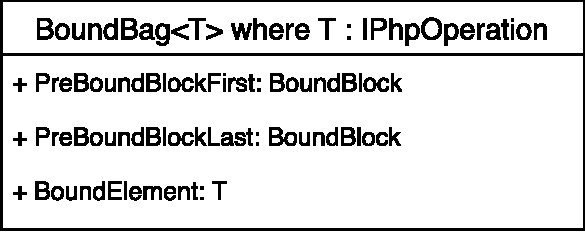
\includegraphics[scale=0.75]{../img/5_3_BoundBag}	
	\caption{Bound bag.}
	\label{fig5.3:BoundBag}
\end{figure}

With the container, we need to change the public public API of the \emph{SemanticBinder} so that it exposes methods that return this \emph{bound bag} instead of a plain bound expression or bound statement. We cannot replace the original methods, however. They are not used just externally but also internally by the \emph{SemanticBinder}. It uses them to bind individual nodes one by one when it is asked to bind a whole expression tree. And in these situations we want them to return plain old bound elements. More about that later.

Instead, we can make the original methods private and add new public methods, let us call them \emph{BindWholeStatement} and \emph{BindWholeExpression}, that will return a \emph{bound bag}. For now, they can call the private ones and only wrap their results into \emph{bound bags} with empty \emph{pre-bound graphs} (\autoref{fig5.3:BindWholeExpr}). We will get back to them later too. Before that, however, we need to fix all the external calls to the - now private - methods and change them to accept a bound bag instead of a sole bound item

\begin{figure}[h]
	\centering	
	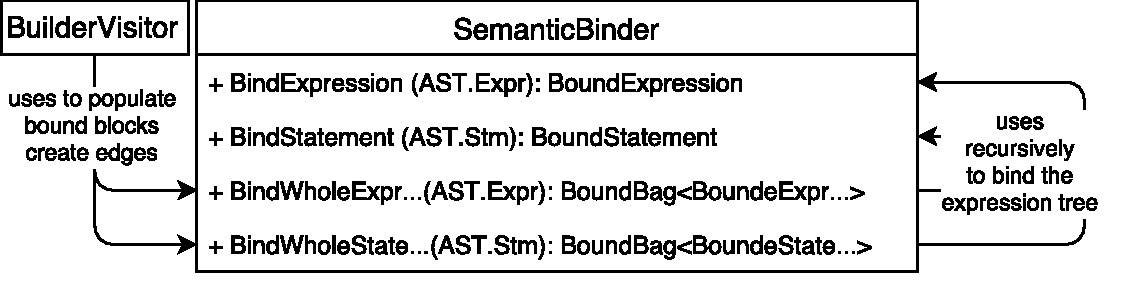
\includegraphics[scale=0.75]{../img/5_3_BoundWholeExpression}	
	\caption{Builder visitor's and semantic binder's relationship.}
	\label{fig5.3:BindWholeExpr}
\end{figure}

The fix is straightforward for statements. The original \emph{BindStatement} method is externally called just once, when the \emph{BuilderVisitor} needs to bind a new statement to add it to its \emph{current bound block}. To support getting a \emph{bound bag} instead of plain bound statement we need to connect its \emph{pre-bound graph} before adding the bound statement to the \emph{current block}. That means creating a simple edge between the \emph{current block} and the \emph{first pre-bound block}, and setting the \emph{last pre-bound block} as the new \emph{current block} (\autoref{fig5.3:BindNewStm}). As the one, into which the bound element will get added.

\begin{figure}[h]
	\centering	
	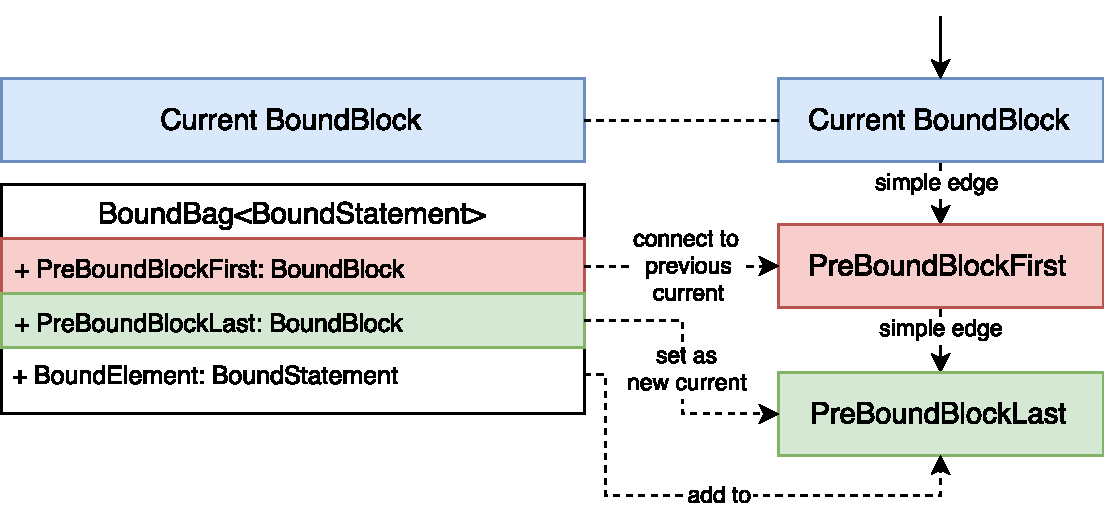
\includegraphics[scale=0.75]{../img/5_3_newStatement}	
	\caption{Connecting a bound bag as a new statement.}
	\label{fig5.3:BindNewStm}
\end{figure}

The situation regarding expressions is a bit more complicated. \emph{BindExpression} is externally called in three situations. When another symbol needs to bind a constant, for example a parameter its initializer. When a \emph{BuilderVisitor} needs an expression representing a reference to a synthesized but user accessible variable, such as \emph{foreach}’s key and value variables. And lastly, when also a \emph{BuilderVisitor} needs to bind an expression for some edge, like a \emph{condition expression} for \emph{condition edge}.

The first two cases are relatively easy to adapt to the bound bag. Both variable references and constants are guaranteed to not to include a \emph{yield} and thus to not to produce a \emph{pre-bound graph}. Therefore, we can retrieve the bound expression from their bound bags and leave the implementation without any further modifications.

The third one is a bit more complicated. There are four instances in which the \emph{BuilderVisitor} asks the \emph{SemanticBinder} to bind a full unrestricted expression. For a \emph{switch edge}’s switch and case values, \emph{condition edge}’s condition, and \emph{foreach}’s enumeree. All of them are problematic because when new edges are being created, it is hard to say what the \emph{current bond block}, to which the \emph{pre-bound graph} should be connected, actually is.

Generally, there are two possible answers for that. One is enriching each of these edges with special branches for these expressions’ pre-bound blocks. On one hand, this is more systematic, it clearly maps the intend to the semantic structure. On the other, it increases complexity for all of these edges’ instances to support a feature used only by generator methods. The second way is to choose any appropriate block and connect the \emph{pre-bound graph} to it. An appropriate block means any block that the \emph{pre-bound graph} can be connected to with the condition that emit of the result must produce a program with correct PHP semantics.

For \emph{condition edge}’s condition, \emph{foreach}’s enumeree, and \emph{switch}’s switch value expressions one such block is their edge’s \emph{source block}. That it the block, the edges connect to as their starting point and also usually the last \emph{current block}. It is a good choice, because these expressions are the first things executed within their respective edges and so the block directly before said edges is also a block directly before them.

Thus, for these three the solution is to take the \emph{first pre-bound block}, connect it to the edge’s \emph{source block}, set the \emph{last pre-bound block} as the new \emph{source block} (\autoref{fig5.3:BindIfEdge}), and continue the edge creation using a bound expression as before.

\begin{figure}[h]
	\centering	
	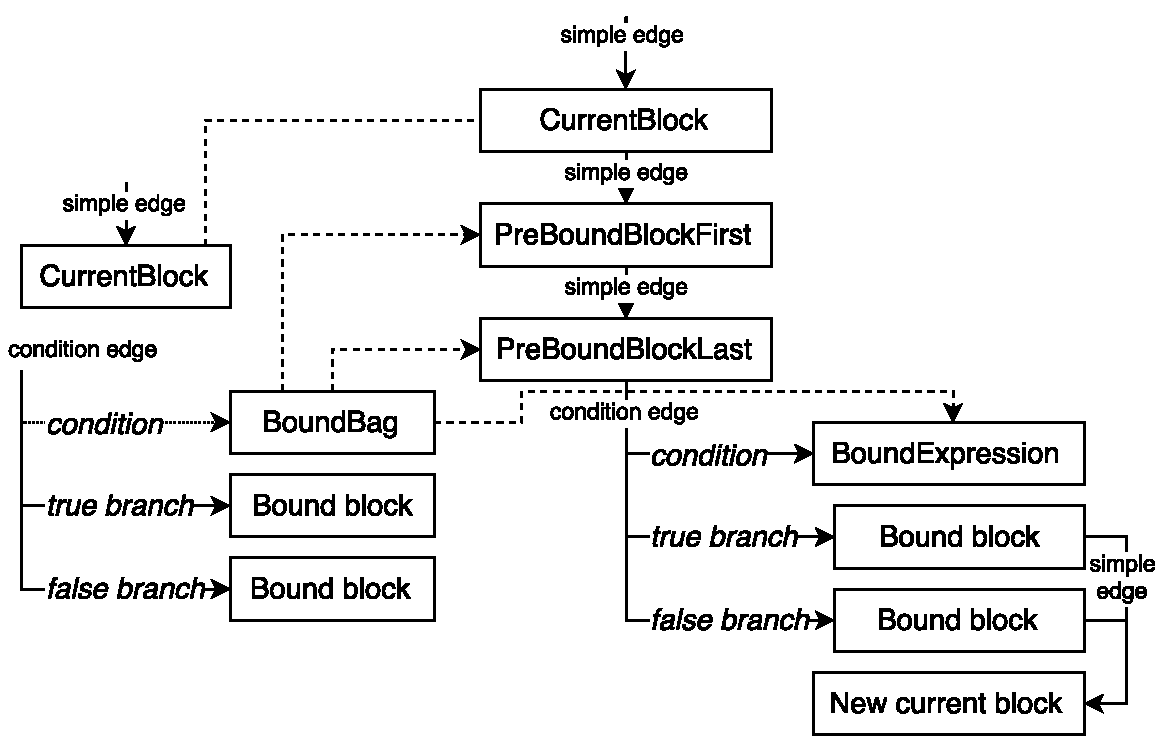
\includegraphics[scale=0.70]{../img/5_3_newInIfEdge}	
	\caption{Connecting a bound bag as a condition edge's condition.}
	\label{fig5.3:BindIfEdge}
\end{figure}

This approach is, unfortunately, not applicable for the fourth case, a \emph{switch edge}’s (\autoref{fig5.3:SwitchEdge}) case value expression. This is an expression representing the value a \emph{switch value} is compared to for each case block. The reason is, that the \emph{case value expression} is executed neither in the beginning of the edge or directly after some other block, so there is simply no block to connect the \emph{case value}’s \emph{pre-bound graph} to. With it we need to go the first way and implement a support for \emph{pre-bound blocks} directly on the edge. Actually, not on the edge itself but on the \emph{case block} the \emph{switch edge} points to.

\begin{figure}[h]
	\centering	
	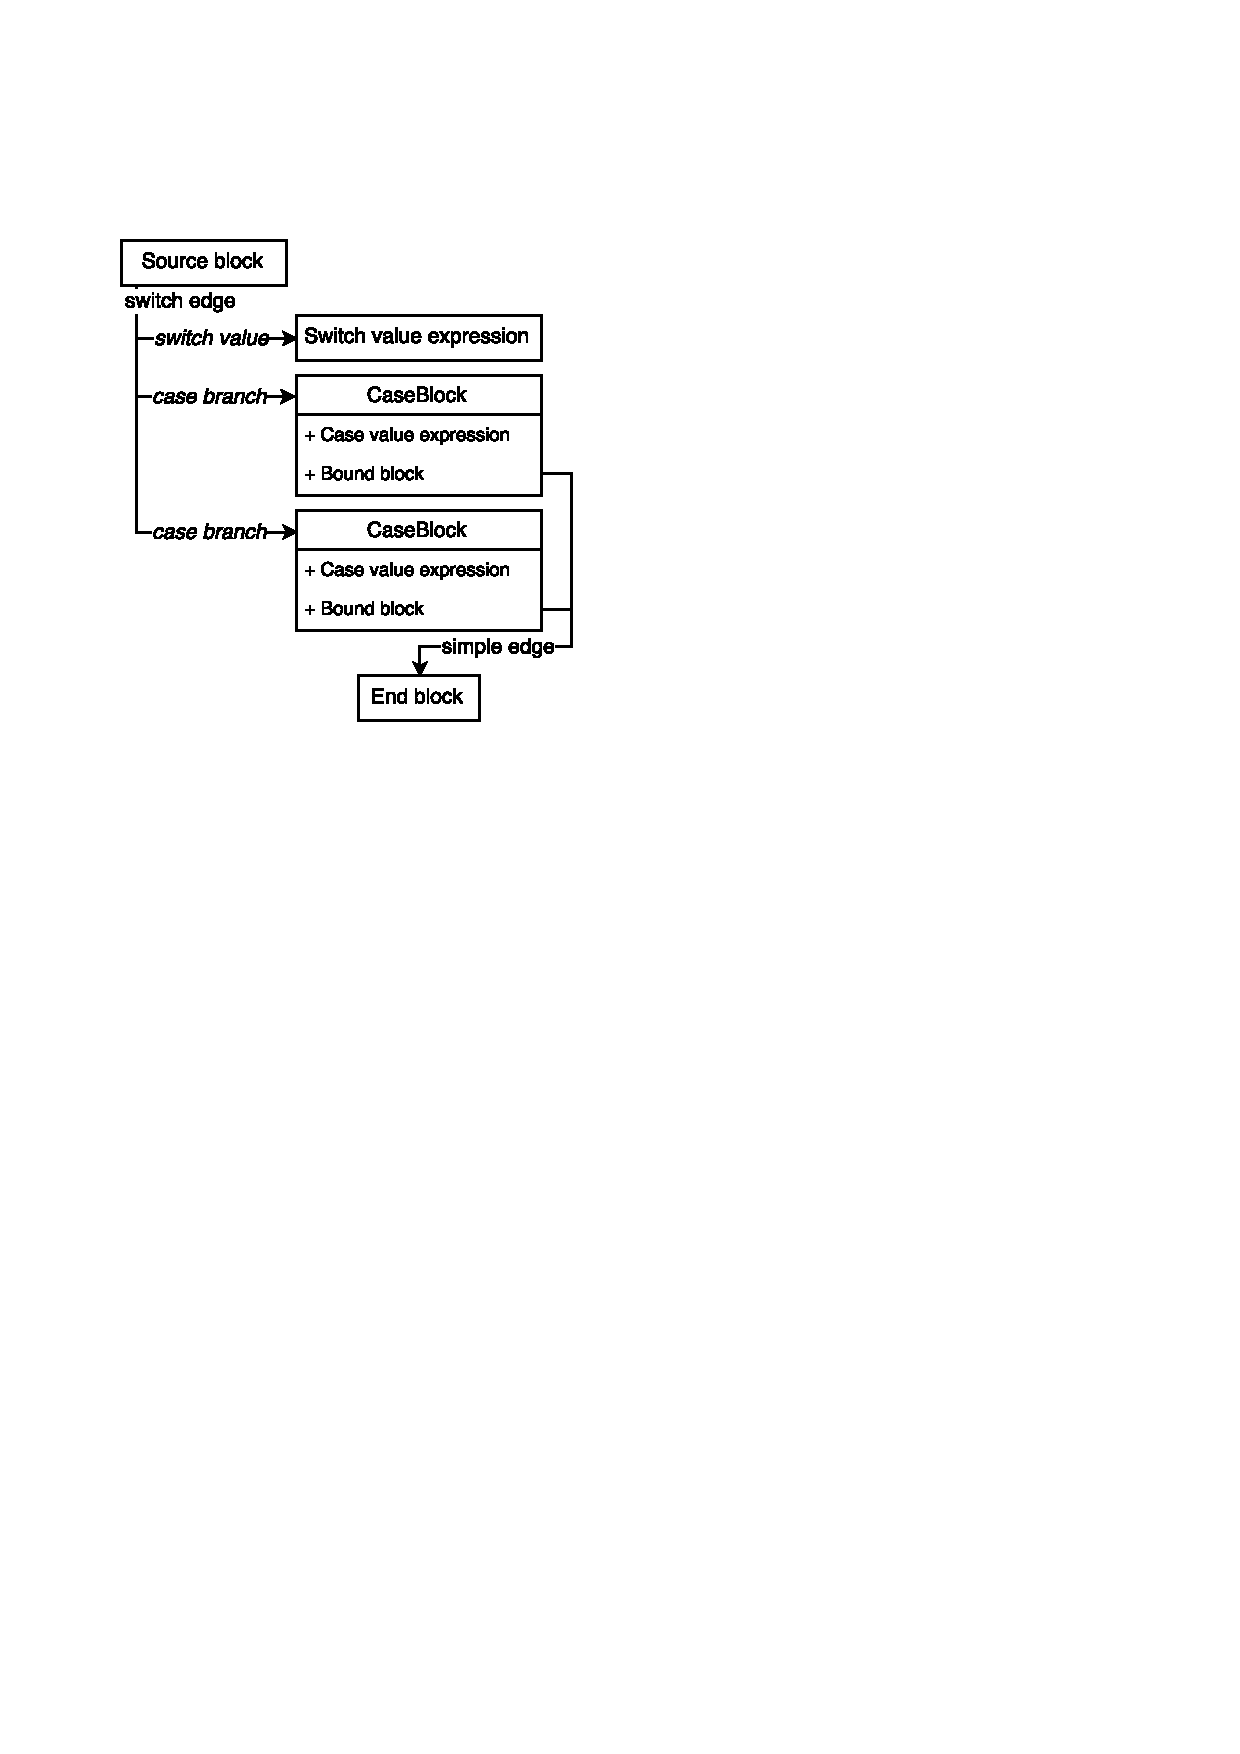
\includegraphics[scale=0.75]{../img/5_3_switchEdge}	
	\caption{Switch edge diagram.}
	\label{fig5.3:SwitchEdge}
\end{figure}

That itself is not that complicated. We can remember the whole case value bound bag in the case block and emit the \emph{pre-bound graph} directly before the case value condition. The issue is, that the evaluation stack is not guaranteed and actually never is empty at that point. Because only one case block can be taken in PHP switch, Peachpie actually keeps the \emph{switch value} on the evaluation stack from the beginning of a switch edge evaluation and goes one \emph{case block} after another comparing their \emph{case values} with it.

Therefore, if a particular case block has any \emph{pre-bound graph} we need to pop the \emph{switch value} first and then, after emitting its \emph{pre-bound graph}, load it again. To not to evaluate the \emph{switch value} multiple times, we also must replace it with a temporal variable. A temporal variable into which the \emph{switch value} is saved, or captured in other words, in the very beginning.

There are certain optimizations that can be done as part of this process. For example, we do not need to do the whole switch value saving if it is a constant. They are, however, implementation details. 

\subsection{Capturing branches with yields}

Now that all external components can handle bound bags with pre-bound blocks, it is time to actually implement the algorithm that creates them. The implementation is based on one core principle. 

When the semantic binder is asked to bind an AST, be it an expression or a statement, it first of all prepares an empty \emph{first pre-bound block} for the item that will be bound. Then, it proceeds with binding the element, its children, and so on recursively as already described in the semantic graph chapter. And when any of these nodes is under any path between a \emph{yield} and the root of the currently bound expression tree, it creates its semantic representation but does not simply return it. Instead, the semantic binder constructs a new \emph{assignment statement} that sets the bound expression to a new temporal variable, puts said statement into the current \emph{pre-bound block}, and returns a \emph{read expression} from the temporal variable (\autoref{fig5.3:CaptureWithYield}). That way the read from the temporal variable ends up in the resulting expression tree instead of the bound expression and the bound expression becomes captured. And when the AST finishes binding it gets returned as part of the bound bag’s pre-bound graph.

\begin{figure}[h]
	\centering	
	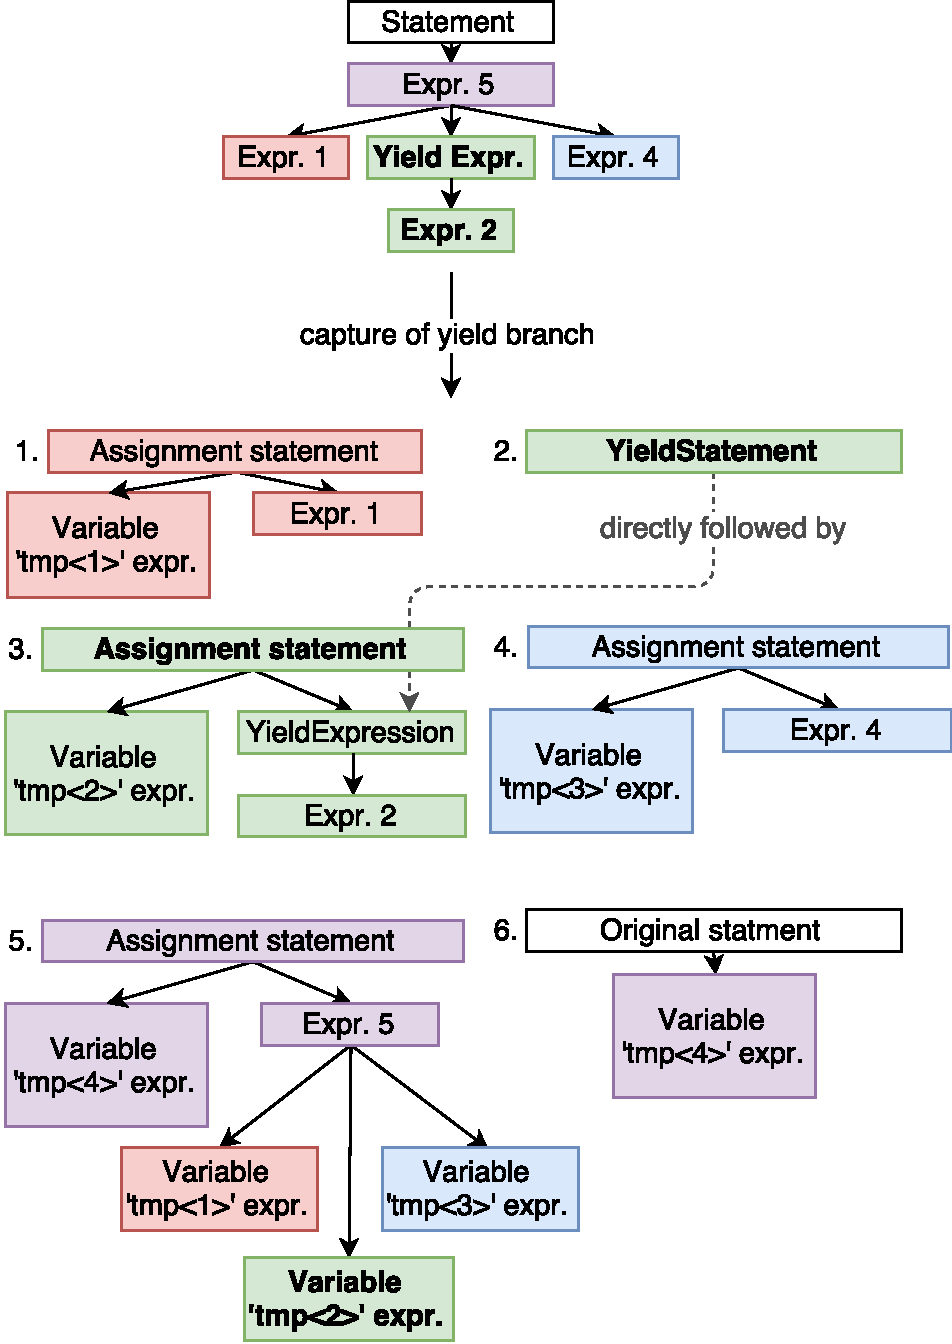
\includegraphics[scale=0.75]{../img/5_3_branchesWithYields}	
	\caption{Capturing a branch with a yield.}
	\label{fig5.3:CaptureWithYield}
\end{figure}

Two things are needed to support such behavior, the ability to determine whether any particular node is under a path between the current expression tree’s root a \emph{yield} and a way to keep \emph{pre-bound blocks} while an expression tree for an AST is being binded. Before going into details on implementing each of these, however, let us first take a look at a small modification we have made to the algorithm in comparison to the one described in a previous chapter\footnote{Chapter \ref{AlghTheory}}.

\subsection{Correctness of modified capturing algorithm}

The actually implemented algorithm captures all branches that start with children of elements on the \emph{root-yield} path instead of only the children to the left. It also captures branches starting on the path itself, after all they are children of some elements one level higher in the path. The reason for that is, that neither the AST nor the semantic tree has a generic notion of left to right ordered children. Therefore it would be hard to determine whether a current element is to the left of the path or to the right. This change, however, does not alter the fact that the transformation keeps the original order of execution.

The implemented version captures a superset of branches the theoretical algorithm did. The ones on top of that are, as the original were, still captured and prepended in a post-order, which guarantees the correct order of execution. In essence, the ones to the right will get prepended and thus executed only after those to the left, and the ones on the path itself only after all their children.

The capturing is done in a post-order order because following statement holds true. The \emph{SemanticBinder} itself operates as a depth first search and the capturing is the last part of a node’s binding process. When an element is being bound, its semantic representation is created first, part of which is fully binding its children from left to right, and only after that, the node itself might get captured and subsequently returned as bound. The thing is, that as part of the children's’ binding process, they themselves might get captured and therefore prepended first. 

Capturing both a child node and its parent’s, which is something that happens with our version for almost all elements on the path, is not a problem either. It creates two prepended statements, first the child’s and then the the parent’s as proven above. The parent’s prepended statement will contain an expression tree with the children’s original branch replaced by the children’s temporal variable (\autoref{fig5.3:CaptureWithYield}). And the original expression tree will contain the parent’s branch replaced with the parent’s temporal variable. Since the children’s prepended statement is first, it will get executed before the parent’s. Thus the execution order will remain correct.

\subsection{Creating and keeping the pre-bound graph}

\begin{figure}[h]
	\centering	
	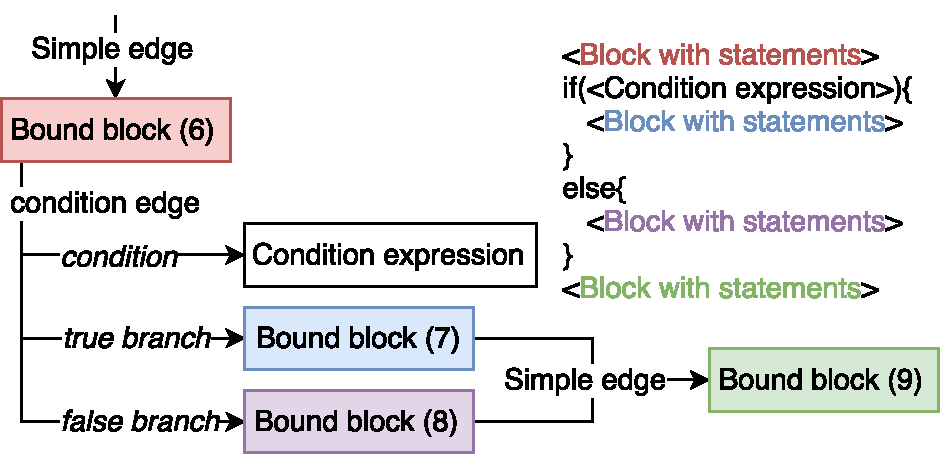
\includegraphics[scale=0.75]{../img/5_3_blockOrdinal}	
	\caption{Ordinal number of bound blocks.}
	\label{fig5.3:BlocksOrdinal}
\end{figure}

\subsection{Path between the root and yields}

\begin{figure}[h]
	\centering	
	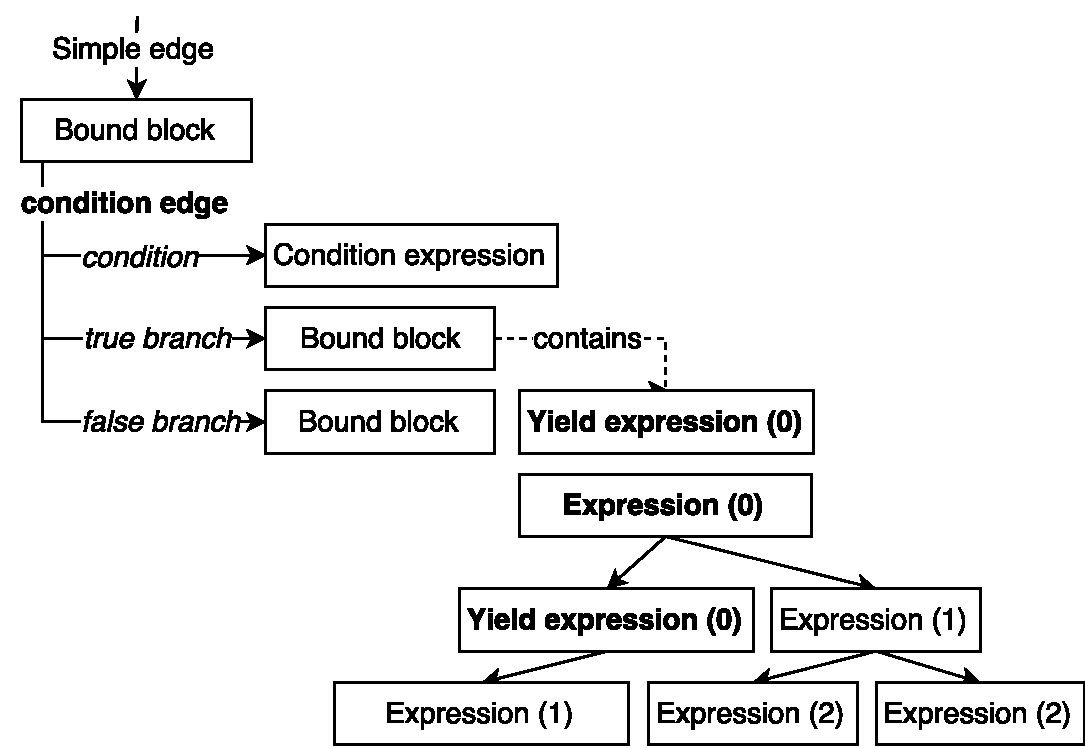
\includegraphics[scale=0.75]{../img/5_3_path}	
	\caption{Path between a yield and expression tree's root.}
	\label{fig5.3:Path}
\end{figure}

\subsection{Conditioned branches}

\begin{figure}[h]
	\centering	
	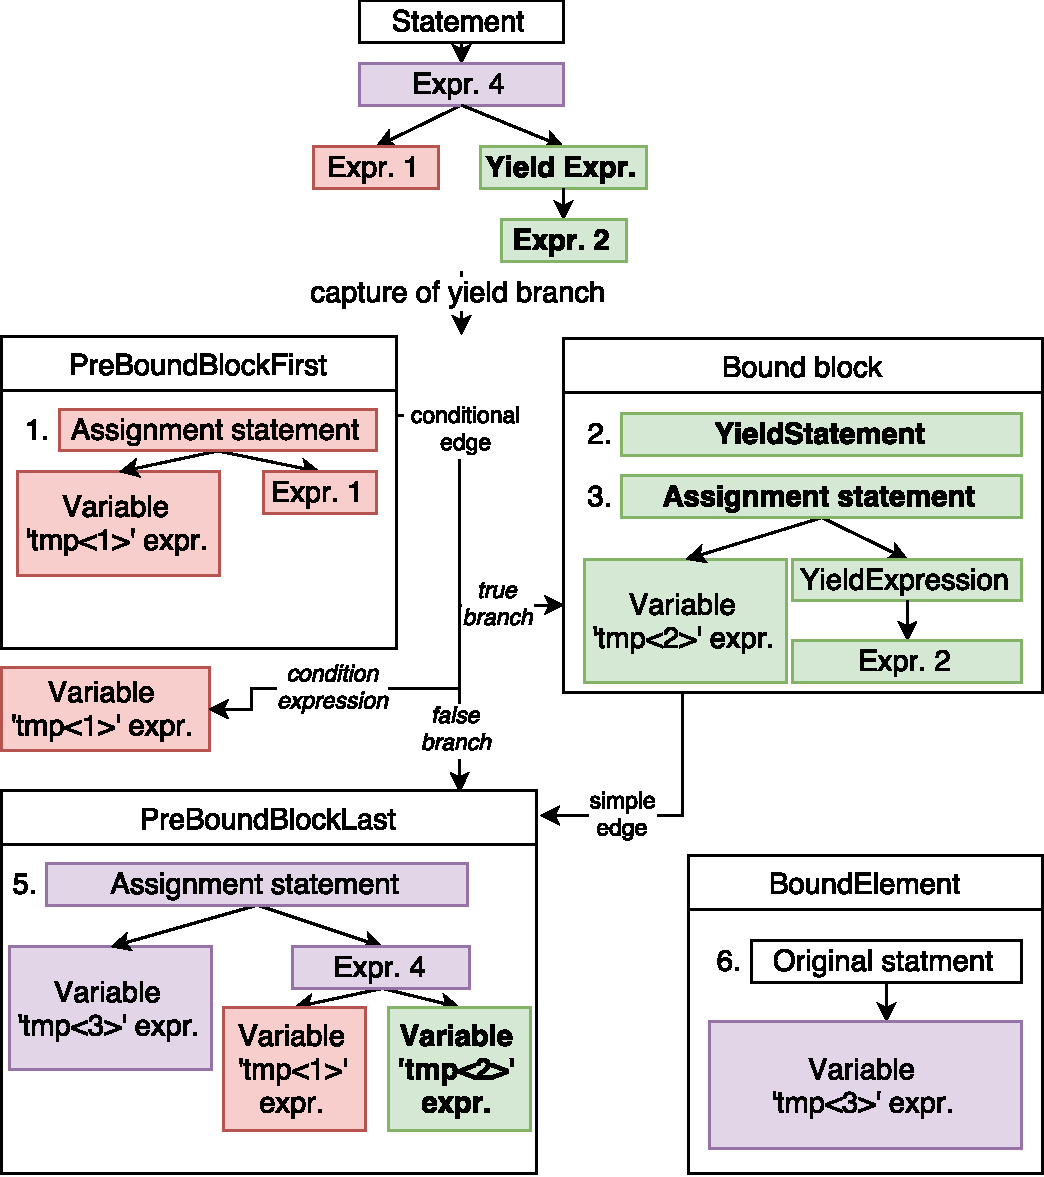
\includegraphics[scale=0.75]{../img/5_3_yieldInCond}	
	\caption{Capturing a yield in a conditioned branch.}
	\label{fig5.3:YieldInCond}
\end{figure}

\subsection{Implementation remarks}

\section{Yield in exception handling blocks}

\subsection{Yields and exception handling blocks in PHP}

\subsection{Solution in Peachpie}

\section{Future work}

Even though this thesis comes with a full featured implementation, there is obviously a room for further expansion. And since the project is, as of writing this thesis, still in a rapid development, it is not only possible but very probable that many of these possible follow ups will get implemented soon. That, however, does not mean they should not be noted here.

In addition to implementing the aforementioned yields in exception handling blocks, the other largest opportunity for improvement lies in employing lowering more throughout the compiler. Both the yield statement and the yield expression could be largely replaced by a lowering into lower level language constructs (\autoref{fig5.5:YieldInCond}). While having standalone nodes was very useful for prototyping and debugging reasons, using already existing means, the rest of the infrastructure understand, is better in the long run. 

\begin{figure}[h]
	\centering	
	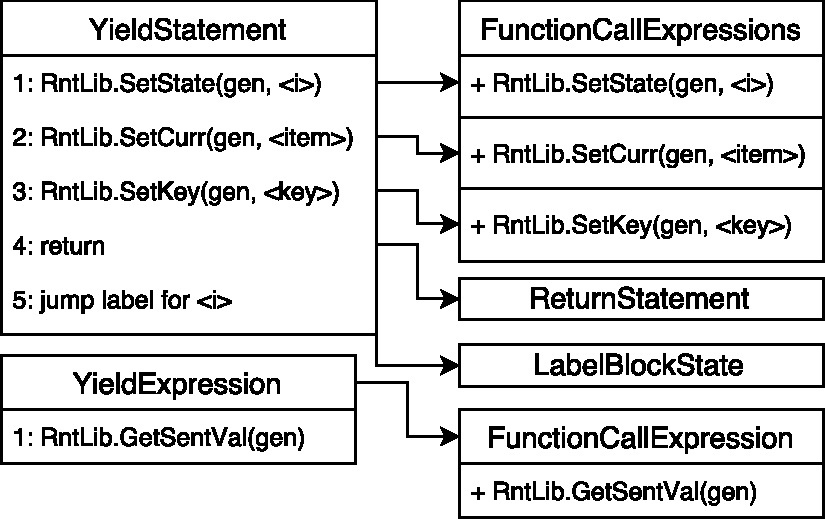
\includegraphics[scale=0.75]{../img/6_6_yieldLowering}	
	\caption{Possible lowering solution to a yield expression and a yield statement.}
	\label{fig5.5:YieldInCond}
\end{figure}

Lowering could also be used instead of having a custom path in the emit method of a routine symbol for generators\footnote{Chapter \ref{MethdSymbol}}. For generator methods, the semantic binder could simply do two things. First, construct a semantic graph that would represent a generator’s instantiation, initialization, and return and then use the graph as the body of the actual generator method. Second, synthesize a separate routine symbol for the generator's next method and bind the original generator method’s body for it.

While not particularly interesting or complex, a \emph{yield from} statement could also be implemented. It provides a way to specify that at some point a generator should yield elements from some iterator until it exhausts it and only then move on to the next \emph{yield}.

There is also great potential in expanding the available code diagnostics. Peachpie compiler could, for example, warn about using \emph{yield}s in finally block, short-circuit evaluated branches, or other potentially problematic places.


